% !TeX root = ../report_project_carac_sky130A.tex

\section{Standard 1.8-V MOS Characterization}
\label{sec:01v8_mos_characterization}


% ============================================================
% Device under test
% ============================================================

\subsection{Device Under Test}

The standard \qty{1.8}{\volt} devices are

\begin{center}
	\code{sky130\_fd\_pr\_\_nfet\_01v8}
	\qquad and \qquad
	\code{sky130\_fd\_pr\_\_pfet\_01v8}.
\end{center}

Unless otherwise stated,

\begin{equation}
	W=\qty{10}{\micro\metre},
	\qquad
	L=\qty{0.5}{\micro\metre}.
\end{equation}

All results correspond to TT at \qty{27}{\degreeCelsius}.


% ============================================================
% Drain current
% ============================================================

\subsection{Drain Current Characteristics}


% ------------------------------------------------------------
% Transfer
% ------------------------------------------------------------

\subsubsection{Transfer Characteristics}

The transfer characteristic provides a direct reference for gate bias
and available current at

\begin{equation}
	|V_{DS}|=\qty{0.9}{\volt}.
\end{equation}

\begin{figure}[H]
	\centering
	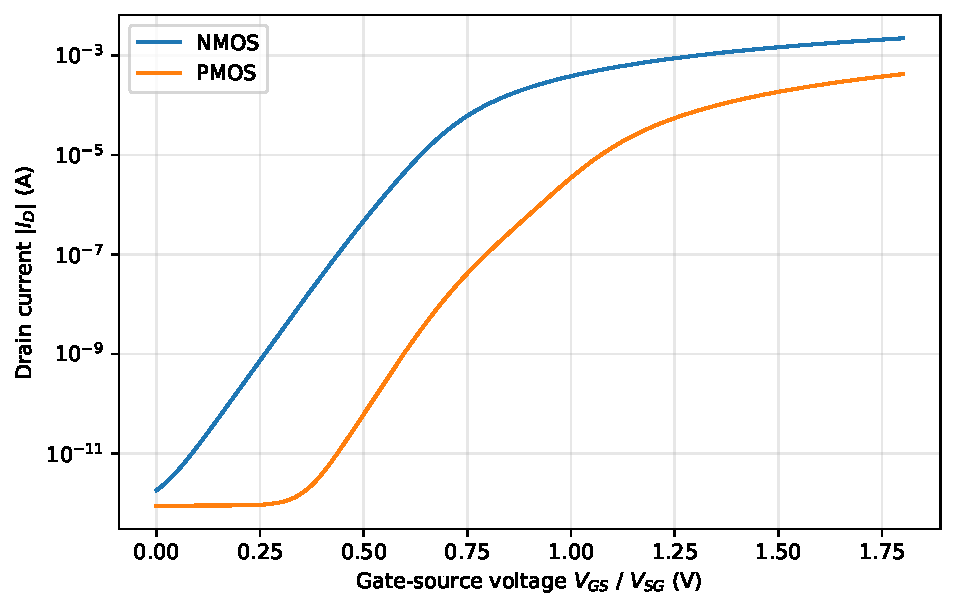
\includegraphics[width=0.72\textwidth]
	{figures/mos_dc/id_vs_vg_01v8.pdf}
	\caption{Drain-current transfer characteristics of the standard
		\qty{1.8}{\volt} NMOS and PMOS devices.}
	\label{fig:id_vs_vg_01v8}
\end{figure}

For equal geometry and gate-voltage magnitude, the NMOS provides
significantly higher current than the PMOS.


% ------------------------------------------------------------
% Output
% ------------------------------------------------------------

\subsubsection{Output Characteristics}

The output-characteristic families provide a direct reference for
current capability and saturation behaviour.

\begin{figure}[H]
	\centering
	
	\begin{minipage}[t]{0.49\textwidth}
		\centering
		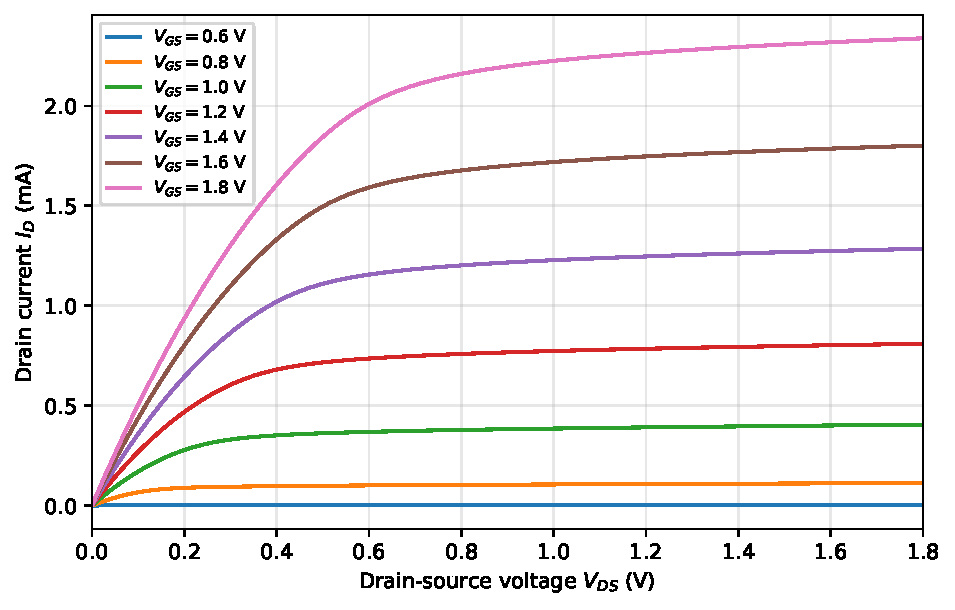
\includegraphics[width=\linewidth]
		{figures/mos_dc/id_vs_vds_01v8_nmos.pdf}
		
		\smallskip
		\small (a) NMOS
	\end{minipage}
	\hfill
	\begin{minipage}[t]{0.49\textwidth}
		\centering
		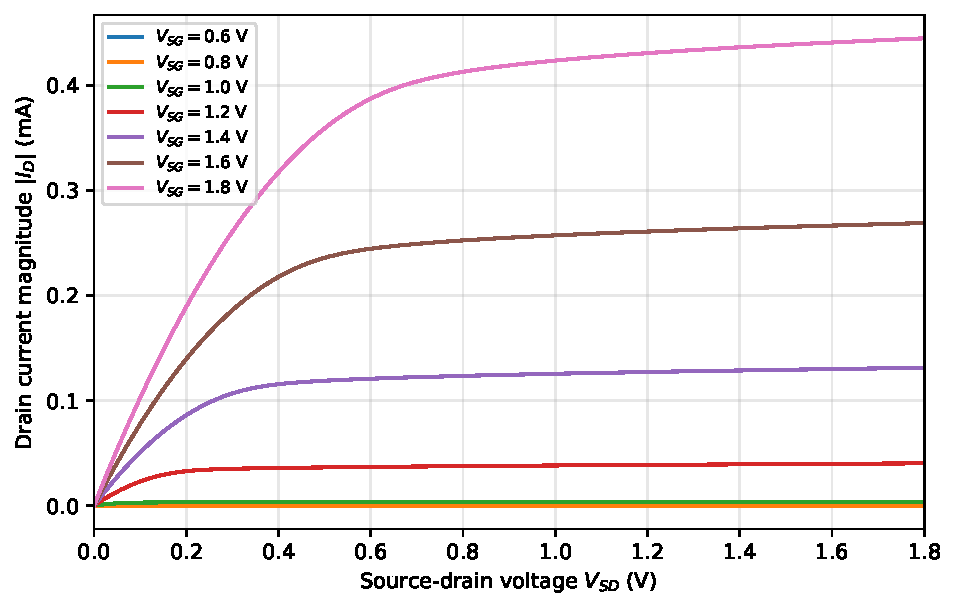
\includegraphics[width=\linewidth]
		{figures/mos_dc/id_vs_vsd_01v8_pmos.pdf}
		
		\smallskip
		\small (b) PMOS
	\end{minipage}
	
	\caption{Output-characteristic families of the standard
		\qty{1.8}{\volt} MOS devices for gate-voltage magnitudes from
		\qty{0.6}{\volt} to \qty{1.8}{\volt}.}
	\label{fig:output_01v8}
\end{figure}

At the highest gate bias, the NMOS current is approximately five times
larger than the PMOS current for the same geometry.


% ============================================================
% Threshold and saturation
% ============================================================

\subsection{Threshold and Saturation Voltages}


% ------------------------------------------------------------
% Threshold
% ------------------------------------------------------------

\subsubsection{Threshold Voltage}

At $|V_{DS}|=\qty{0.9}{\volt}$ and $V_{SB}=0$, the compact-model
operating-point data give approximately:

\begin{table}[H]
	\centering
	\small
	\caption{Threshold voltages for the reference
		\qty{1.8}{\volt} devices.}
	\label{tab:vth_01v8}
	
	\begin{tabular}{lcc}
		\toprule
		Device & $W/L$ ($\mu$m/$\mu$m) & $|V_{TH}|$ \\
		\midrule
		
		NMOS & 10/0.5 & \qty{0.61}{\volt} \\
		PMOS & 10/0.5 & \qty{0.99}{\volt} \\
		
		\bottomrule
	\end{tabular}
\end{table}

The geometry dependence of $V_{TH}$ and the bias dependence of
$V_{DSAT}$ are shown together in
Figure~\ref{fig:vth_vdsat_01v8}.

\begin{figure}[H]
	\centering
	
	\begin{minipage}[t]{0.49\textwidth}
		\centering
		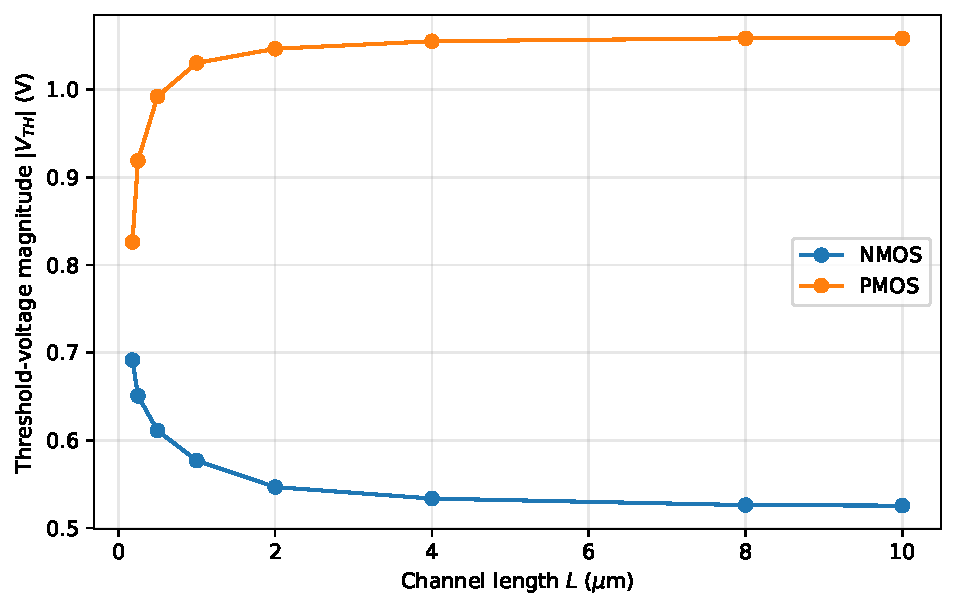
\includegraphics[width=\linewidth]
		{figures/mos_dc/vth_vs_length_01v8.pdf}
		
		\smallskip
		\small (a) Threshold voltage versus $L$
	\end{minipage}
	\hfill
	\begin{minipage}[t]{0.49\textwidth}
		\centering
		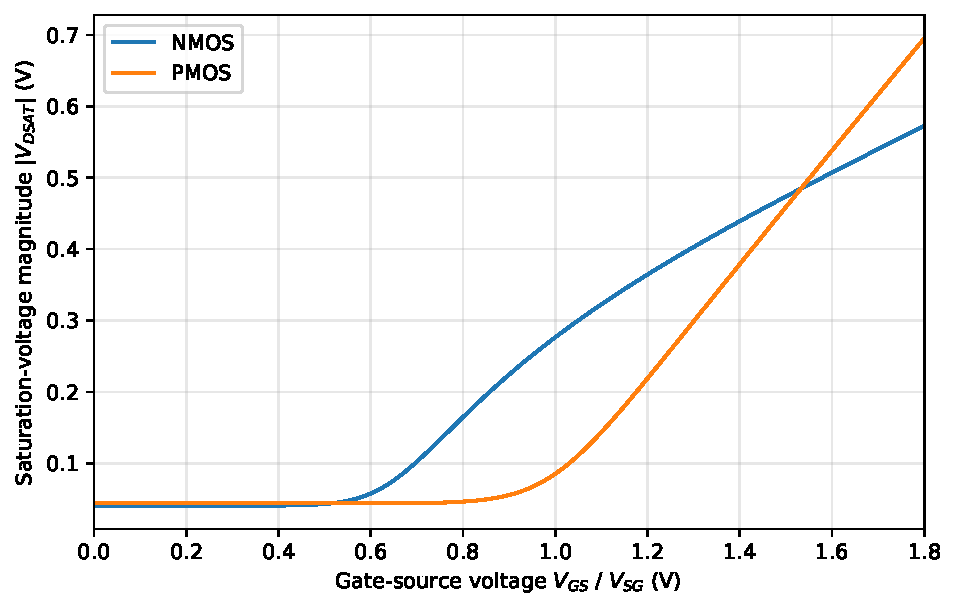
\includegraphics[width=\linewidth]
		{figures/mos_dc/vdsat_vs_vg_01v8.pdf}
		
		\smallskip
		\small (b) Saturation voltage versus gate bias
	\end{minipage}
	
	\caption{Threshold- and saturation-voltage characteristics of the
		standard \qty{1.8}{\volt} devices.}
	\label{fig:vth_vdsat_01v8}
\end{figure}

The NMOS threshold decreases with increasing channel length, whereas
the PMOS threshold magnitude increases toward approximately
\qty{1.06}{\volt}.

The $V_{DSAT}$ characteristic provides a direct headroom reference for
future bias selection.


% ============================================================
% gm/ID
% ============================================================

\subsection{Transconductance Efficiency}

The $g_m/I_D$ characteristic is retained as the main sizing-oriented
result. Drain current is normalized by width so that the curve can be
used independently of the reference transistor width.

\begin{figure}[H]
	\centering
	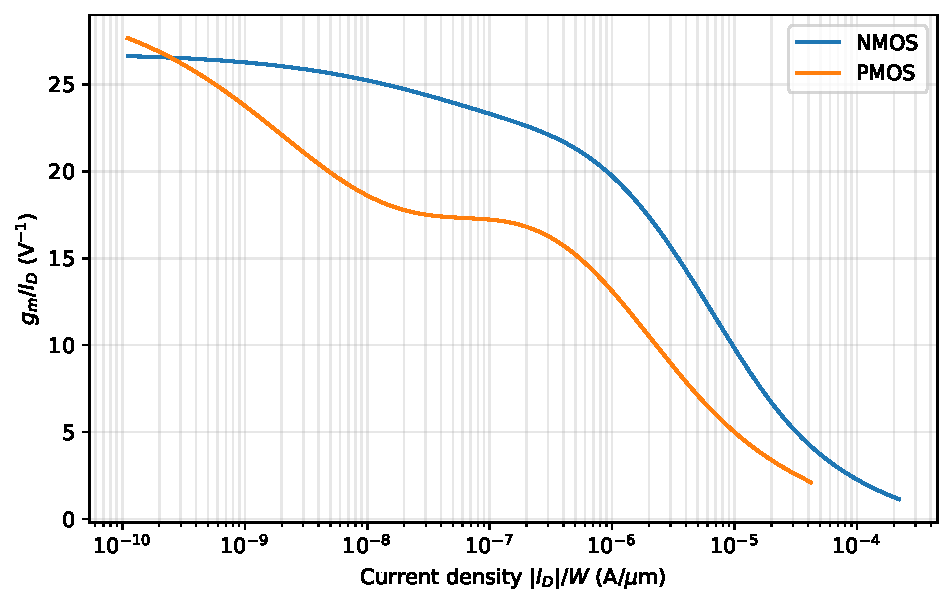
\includegraphics[width=0.72\textwidth]
	{figures/mos_dc/gmid_vs_current_density_01v8.pdf}
	\caption{Transconductance efficiency $g_m/I_D$ versus
		drain-current density $|I_D|/W$.}
	\label{fig:gmid_vs_current_density_01v8}
\end{figure}


% ============================================================
% Capacitance
% ============================================================

\subsection{Gate Capacitance}

The effective gate capacitance is characterized at
\qty{1}{\mega\hertz} as a function of bias and geometry.

\begin{figure}[H]
	\centering
	
	\begin{minipage}[t]{0.49\textwidth}
		\centering
		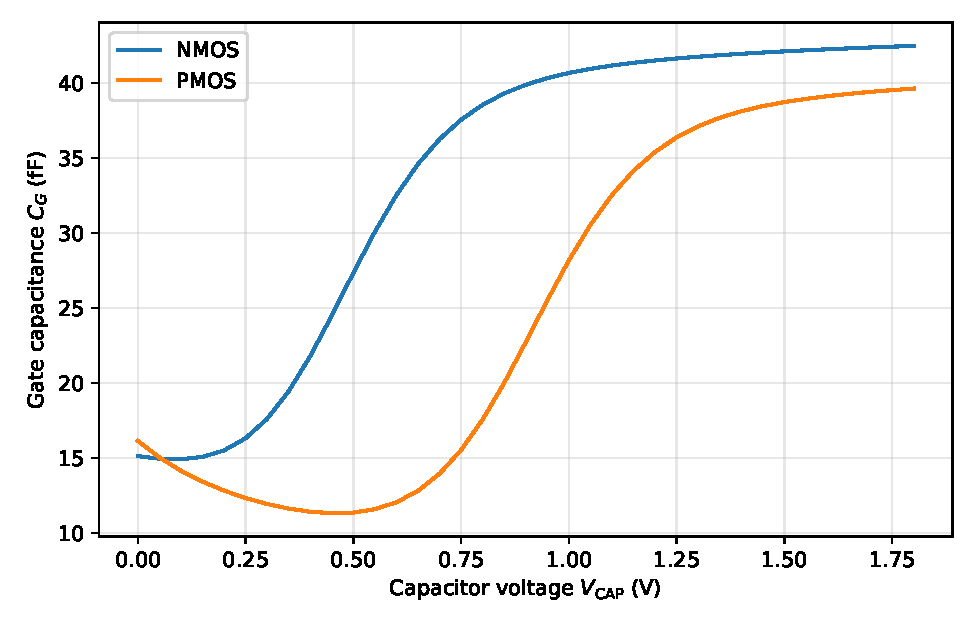
\includegraphics[width=\linewidth]
		{figures/moscap/moscap_cv_01v8.pdf}
		
		\smallskip
		\small (a) Bias dependence
	\end{minipage}
	\hfill
	\begin{minipage}[t]{0.49\textwidth}
		\centering
		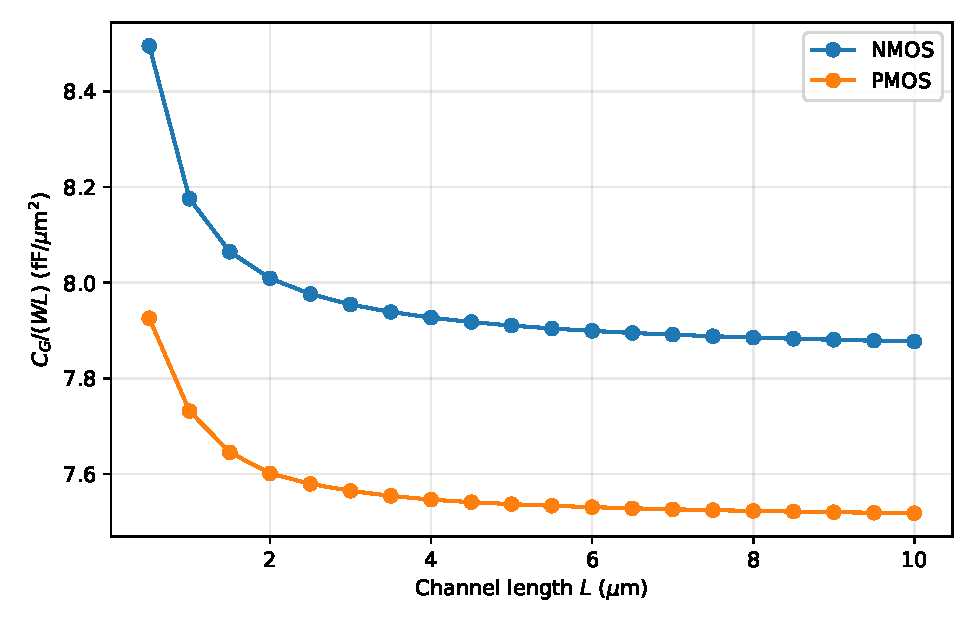
\includegraphics[width=\linewidth]
		{figures/moscap/moscap_density_vs_l_01v8.pdf}
		
		\smallskip
		\small (b) Geometry dependence
	\end{minipage}
	
	\caption{Effective gate-capacitance characteristics of the standard
		\qty{1.8}{\volt} NMOS and PMOS devices.}
	\label{fig:moscap_01v8}
\end{figure}

At long channel lengths, the extracted capacitance density approaches
approximately
\qty{7.9}{\femto\farad\per\micro\metre\squared} for the NMOS and
\qty{7.5}{\femto\farad\per\micro\metre\squared} for the PMOS.

The larger normalized capacitance observed for short devices reflects
the greater relative contribution of edge and overlap capacitances.